\documentclass[a4paper]{dnd5}
\usepackage{wrapfig}

\newcommand\inc[1]{
 \includegraphics[width=0.22\textwidth, height=0.22\textwidth]{#1}
}


\newcommand\origin{\textbf{Origin:}}
\newcommand\sigil{\textbf{Sigil:}}
\newcommand\words{\textbf{Words:}}

\pagestyle{fancy}

\newtoggle{DM}
%\toggletrue{DM}
\togglefalse{DM}



\iftoggle{DM}{
  \lhead{DM's Version}
}{
}


\begin{document}


\section*{De natura umbra Druchii}

Since the Sundering of the Elves, the Druchii, also known as the Dark Elves have lived in Nagaroth, by all accounts an icy hell.  They have given themselves unto debauchery and depravity, ritual madness and religious ecstasy.  

\begin{wrapfigure}{r}{0.2\textwidth}%
\begin{center}%
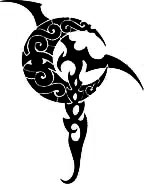
\includegraphics[width=0.12\textwidth,height=0.2\textwidth]{darkelf_logo.jpg}%
\end{center}%
\end{wrapfigure}

Their countryside is bleak.  Populated by short-lived slaves working in mines, minding herds of animals or working in leaky fishing-boats.  Their cities have innumerable black towers rising like pinnacles of ice from the cold, hard rock of Nagaroth. Due to the harsh and unforgiving weather, few live outside their vast cities and so the Druchii cities are some of the most densely populated centers in the world.   All of these cities are dark and evil places. Their dungeons are crammed with captives whose wailing fill the air and whose moans seep through the thick walls of the high towers, saturating the place with pain, despair and the souls of the dying. At the tips of these towers, the Sorceresses of Nagaroth cast their malign magic over the world.

The inhabitants of Nagaroth are partitioned based on a strict caste system.  The Druchii themselves are elves.  Their lives are completely focused on zealous theology, military training, and excellence.  The Druchii are born into a noble house.  The standing of a member of the Druchii rises and falls with that of their house.  Periodically there are internal schisms within a house and then two new houses arise from the ashes of the first.  At that time usually one or both new houses are exterminated by internecine actions or intervention by external houses.  

Nagaroth is ruled by the Gomaithri (high council).  Every Druchii of age gets a vote.  The Gomaithri consists of the candidates with the top 23 votes in the nation.  Election rigging is both rife and punishable by death if discovered.  The leader of the council is named the Witch King and he rules with terrible power.

When a child is born, they are examined by members of the Gomaithri from the child's house to see whether they are fit and healthy enough to be allowed to live. The babies are then left in the mountains for several days in a test to die of exposure or survive the ordeal.  As children Druchii undergo a rigorous training and education mandated by the state.  The training involves learning stealth, cultivating loyalty to the Dark Elf nation, military training, pain tolerance, hunting, dancing, singing and social (communicating) preparation.  
The aim of the system is to produce physically and morally strong individuals to serve in the Druchii army. It encourages conformity and the importance of the state over one's personal interest and generates the future elites of Nagaroth.  The Druchii become the \emph{Walls of Nagaroth} because Nagaroth is the only nation in the known world whose cities have no defensive walls after they had been demolished at the order of Melanaigis III.  Discipline is strict and dark elves are encouraged to fight amongst themselves to determine the strongest members of their group.

The children live in groups and during this time are encouraged to give their loyalty to their communal mess hall, rather than to their families. Beginning at the age of 12 children are given only one item of clothing per year — a black cloak.  They are intentionally underfed to encourage them to master the skills necessary to become successful at stealing their food. This lets the children become accustomed to cold and hunger so that during a campaign these are not a problem. They are severely punished, however, if they are caught stealing. 

At around age 12 the children enter formal education.  They board at large military institutions where they train in martial skills, theology, language, magic and science.

 Around the age of 18, the students become reserve members of the Nagaroth army. Some youths are allowed to become part of the Crypteia, a type of \emph{Secret Police}, where they are instructed to spy on the slave population and even kill slaves who are out at night or speak seditiously, to help keep the population submissive.  The state supports this by formally declaring war on the slaves every autumn, so that killing a slave is not regarded as a crime, but a valuable deed for the good of the state.

At the age of 20 or so, the students become full members of the army, although they continue to live in barracks and to compete for a place among the Nagarothi royal guard of honor.  Students are voted into one of the public messes. The voting is done by the members of their mess, and must be unanimous. Rejected candidates can try to gain entry to a different mess for up to ten years. If a member of the Druchii fails to gain entry into a mess by age 30, they become Oistii (non-persons, the word loosely translated means poor in honour). At the age of 30, dark elves are permitted to marry and to become full citizens of Nagaroth who can vote and hold office.  

The Oistii are elves of a lower caste than the Druchii.  Their name means non-people in elvish.  There are a number of ways in which members of the Druchii may become Oistii, for example entire Druchii Houses may be cast down when a member of their house performs some action that is regarded as being unworthy.  This is always fatal for the individual and often for the house, but if the house stands firm they may only be relegated to the ranks of the Oistii.  The Oistii have no voting rights in the Gomaithri and they have severe limitations on the ranks they are legally allowed to hold in the nation.  All Oistii are deemed inferior to any Druchii.

The Awarthii are freed-humans (the name means those who have abandoned - their own people).  They make up a very small proportion of the population.  They are the only people in the nation that are freely allowed to leave Nagaroth.  They are involved with trade with the outside world.  They are always married with children.  The Awarthii report to certain members of the Oistii. In general they have to sail to the Wild Coast or to Northern Cheruskia to find people who will trade with them. They are also involved in smuggling and in the illicit slave trade.

The Guinir are slaves.  They range from state-owned serfs, to slaves who are the personal properties of the houses.   There are no Elven slaves.   There lives are generally short and hard.  They are frequently killed for pleasure.  House slaves may be murdered at any time by any member of the owning house.  There are a number of ceremonies each year where hundreds of slaves are sacrificed to appease the outer gods.  The Guinir outnumber elves by greater than ten to one.  The Druchii live in constant fear of a revolt.  Any insubordination or signs of rebellion are met swiftly and mercilessly.  Slaves are also used to row the galleys, mining, smelting, shepherding, fishing and are fed to the indigenous giant spiders which are kept as pets by the Druchii.

Besides being superb warriors, the dark elves are the preeminent workers of dark magic, particularly blood magic.  Their magic schools are thousands of years old, and they have developed some of the most powerful magical items known to mankind, such as the Speculis Principes Umbras (Mirrors of the Princes of the Shadows), and the Ansible Portarum (Ansible of the Gates).

The so-called dark-elves have given their souls to the old ones.  Their society revolves around the worship of the great ones from beyond the veil.  Truly there can be no redemption for that unfortunate race in this life or the next.  The various religious cults in Nagaroth hold great political power.  Chief amongst these are the worshippers of Lolth, the spider goddess, the watcher in the night, goddess of Suffering, Pain, Death and Disease.  The other cults form an uneasy alliance lest they be destroyed by the followers of Lolth.  Druchii foreign policy exists to further the inscrutable goals of their dark gods.  Other than mass sacrifices, the closest that the Druchii have to a religious ceremony is the annual festival of Melanaigis III, (a deified king of the dark elves) during which a procession, made up of wild female followers, travels through the cities. Some in the procession are armed with sacrificial knives and drag spectators into the streets for summary execution, while others dance or play music. The ``god'' himself is drawn in a chariot, usually by exotic beasts such as lions or tigers. 

It is believed that the Druchii could dominate the entire western half of the known world if it were not for Brythynia, whose armies are great in number and supported by those of Averoigne, Thule and Hibernia. It is said that the dark elves work ceaselessly to weaken the Brythynian empire.  In the face of Brythynian military dominance the Druchii content themselves with raiding the coastal villages on the western seas.  Oft times they send their raiding parties far inland along navigable rivers.  Their most audacious attack to date occurred in AUC 1934 when they sacked Heatherhal, capital of Pict Hibernica.  It was only in the face of a surprise naval victory against part of the Druchii navy and the approaching imperial Brythynian army that the Druchii retreated back across the seas, having burnt the city to the ground, enslaved a fifth of the populace and left corpses of the majority in piles for the gluttonous birds to pick at.  

\end{document}
